\documentclass{article}

\usepackage[margin=1in]{geometry}
\usepackage{setspace}
\usepackage{graphicx}
\usepackage{amsmath}
\usepackage{float}

\title{Final Project Report}
\author{Michael Forney \\ SID: 21392560}

\begin{document}
    \maketitle
    \doublespacing

    \section{Project Overview}
    My final project is a interactive inverse kinematics solver, which can
    generate simple animations by interpolating poses created manually by the
    user, or automatically through inverse kinematics. I used a variation of the
    cyclic coordinate descent algorithm to iteratively improve the parameters of
    the joints, gradually converging on the best solution given a certain set of
    constraints. My project can solve joint structures with arbitrary branching
    at each socket (only outward branching, joints cannot reconnect further down
    in the tree), and both revolute (rotational), and prismatic (translational)
    joints. An example of a structure incorporating all of these features is
    shown on the following page.

    I implemented my project in Haskell, a functional programming language,
    because I noticed that many of the projects we have done in the past were
    suited nicely toward it, because they are mainly computation based, and also
    as a personal challenge. I used Haskell bindings for Gtk+, a common widget
    toolkit, and cairo to render to the canvas area.

    \begin{figure}[H]
        \caption{Main Screenshot}
        \centering
        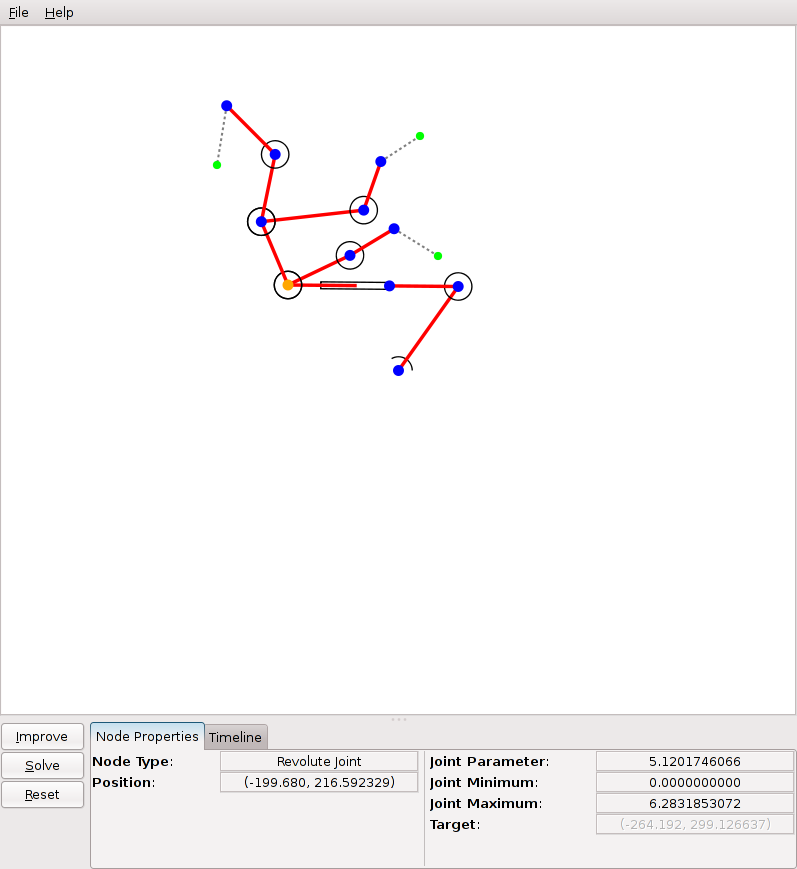
\includegraphics[width=400px]{main_screenshot.png}
    \end{figure}

    There are two major components to my project; the main canvas area where the
    user can manipulate a branching structure of joints, and the timeline tab
    where the user can create an animation and render it, or play it back.

    \subsection{Pose Manipulation}
    In the main canvas area, the user can configure the joint parameters of the
    structure with the mouse, and add or remove target points by double left or
    right clicking. The inverse kinematics problem can then be solved by either
    finding a fixed point of the CCD function, or just performing one step.

    \subsection{Pose Animation}
    In order to create animations, I created a timeline tab, which allows the
    user to set different key frames from a list of saved poses. Poses are then
    interpolated between set key frames, generating a smooth animation. Also, a
    user can create a key frame pose from an interpolated, to perform fine
    adjustments during the course of animating.

    After the key frames are generated, the user can play back the animation
    directly, or, once satisfied, they can render the animation frames to PNG
    images, which can be encoded to video later.

    \begin{figure}[H]
        \caption{Timeline Editor}
        \centering
        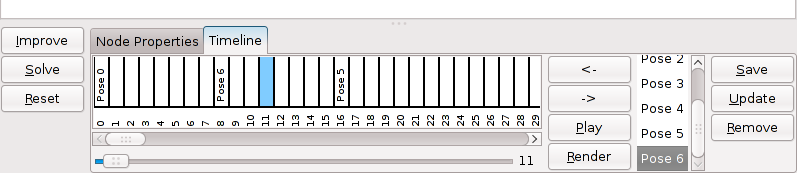
\includegraphics[width=400px]{timeline.png}
    \end{figure}

    \section{Cyclic Coordinate Descent}
    Cyclic coordinate descent is a relatively simple way of iteratively
    improving a structure configuration, gradually converging on a solution. It
    works by first considering joints at the end of arms, and pointing them
    towards the target. Then the parent joint is rotated so that the tip is
    again towards the target. This continues until the root node is reached.
    This process can be repeated multiple times to find a solution to the given
    inverse kinematics problem.
    
    My basic understanding of cyclic coordinate descent came from an article
    written by Ryan Juckett \cite{juckett}. In this article, Jucket explains the
    basic concept, which I took and generalized to more advanced structures. In
    order to allow for branching at sockets, the angle to rotate or position to
    move a joint was not obvious. Also, constraints on joint movement also
    needed to be accounted for.

    \section{Calculating Joint Parameters}
    In order to calculate the parameter of each joint, I used a sum to find the
    sum of squares of the distances between constrained end effectors (rotated
    or translated by some amount), and their target positions. By taking the
    derivative of this sum, I was able to find minimum and maximum points of
    this error, and then use the constraints to find the optimal parameter.

    \subsection{Revolute Joints}
    \begin{figure}[H]
        \caption{Revolute Joint}
        \centering
        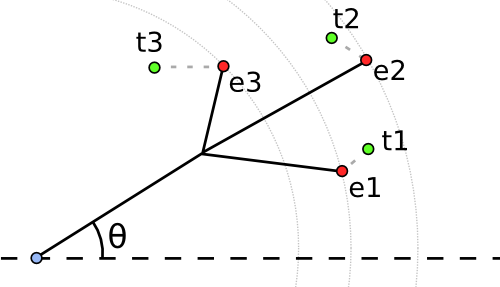
\includegraphics[width=400px]{revolute.png}
    \end{figure}

    In order to minimize the total distance between target end points $t_i$
    and current end points (rotated by some angle $\theta$), $e_i$, I first
    expanded the dot product to simplify the problem.

    \begin{align}
        error &= \sum_{i=1}^n ||t_i - M(\theta) e_i||^2 \\
              &= \sum_{i=1}^n (t_i - M(\theta) e_i) \cdot (t_i - M(\theta) e_i) \\
              &= \sum_{i=1}^n t_i \cdot t_i + (M(\theta) e_i) \cdot
                  (M(\theta) e_i) - 2 t_i \cdot (M(\theta) e_i)
    \end{align}

    \(M(\theta)\) is an orthogonal matrix, so \(||M(\theta) e_i|| = ||e_i||\).
    This makes \(t_i \cdot (M(\theta) e_i)\) the only part of the equation that
    depends on \(\theta\). In order to minimise the error with respect to
    $\theta$, we can maximise this dot product. To find the maximum, I found
    where the derivative was $0$.

    \begin{align}
        0 &= cos(\theta) (t_y e_x - t_x e_y) - sin(\theta) (t_x e_x + t_y e_y) \\
        0 &= cos(\theta) \sum_{i=1}^n
            \left(\begin{smallmatrix}
                0 & 1 \\
                -1 & 0
            \end{smallmatrix}\right) t_i \cdot e_i - sin(\theta) \sum_{i=1}^n t_i \cdot e_i \\
        \theta &= tan^{-1}\left(\frac{\sum_{i=1}^n
            \left(\begin{smallmatrix}
                0 & 1 \\
                -1 & 0
            \end{smallmatrix}\right) t_i \cdot e_i}{\sum_{i=1}^n t_i \cdot e_i}\right)
    \end{align}

    This could either be the maximum or minimum error, and may be out of bounds
    because of the joint constraints, so I use the angle with the smallest error
    out of $\theta$, $\theta + \pi$, $\theta_{min}$, $\theta_{max}$, filtering
    out out of bounds angles.

    \subsection{Prismatic Joints}
    A similar approach was used for prismatic joints which I will not go into.
    The error was a quadratic curve, which had one minimum point, which again
    was compared with the maximum and minimum position.

    \section{Problems Encountered}
    The animation editing panel was the source of many problems for me. It was
    very difficult to keep track of the poses and ensure the user interface was
    in a consistent state. As a result, I had to compromise and make a less
    friendly timeline editor, instead of the drag and drop I had planned.

    It was also quite difficult to keep track of transformations at each joint,
    and to make sure my coordinate systems were consistent when comparing
    points. I was very careful to ensure things were working correctly by
    checking values at each stage against manually calculated values.

    \section{Areas to Expand}
    During the course of implementing my project, there were several areas I
    wanted to take further, but lacked the time. Currently, my project uses
    simple linear interpolation to find poses between key frames. This could be
    expanded to use some curve to preserve continuity between key frames.

    Also, an interactive structure editor to add and remove segments and joints
    would make it easier for users to create a desired figure. My program only
    allows input through a text file, which must be manually created by the
    user.

    My algorithm converged slowly on complex solutions, and although I had an
    idea on how to solve this (first consider constrained points closer to the
    root node, and work outwards, until all constrained nodes are considered), I
    did not have the time to implement my idea.

    \begin{thebibliography}{9}
        \bibitem{juckett}
        Ryan Juckett,
        \emph{Cyclic Coordinate Descent in 2D}.
        Wednesday, 11 February 2009
    \end{thebibliography}

\end{document}

